% !TEX root = poster.tex
%\headerbox{Recent Developments}{name=devs,column=1,row=1,below=run1,above=bottom}{
\headerbox{\textbf{Developments}}{name=devs,column=1,row=1,span=2,below=run1}{
\begin{minipage}{0.474\boxwidth}
\vspace{-2.72em}
\textbf{SS kaon calibration with excited \Bs states}
\vspace{-0.1em}
\begin{itemize}
\item SS kaon taggers calibrated with \BsToDspi only
\begin{itemize}
\setlength{\itemindent}{-.11in}
\item[${\color{tu_gruen}-}$] limited statistics
\item[${\color{tu_gruen}-}$] time-dependent analysis required
\end{itemize}
\vspace{-0.8em}
\item new idea: calibrate with $B_s^{**0}$ decays
%\setlength{\itemindent}{.05in}
%\item[${\color{tu_gruen}\Rightarrow}$] further control channel for SS kaon tagging
\begin{itemize}
\setlength\itemsep{0.01em}
\setlength{\itemindent}{-.11in}
\item[${\color{tu_gruen}-}$] narrow states
\item[${\color{tu_gruen}-}$] reconstruct in  $B_s^{**0}\to\Bp\Km$ decays
\item[${\color{tu_gruen}-}$] calibrate by counting, as in other charged modes 
\end{itemize}
\end{itemize}
\begin{center}
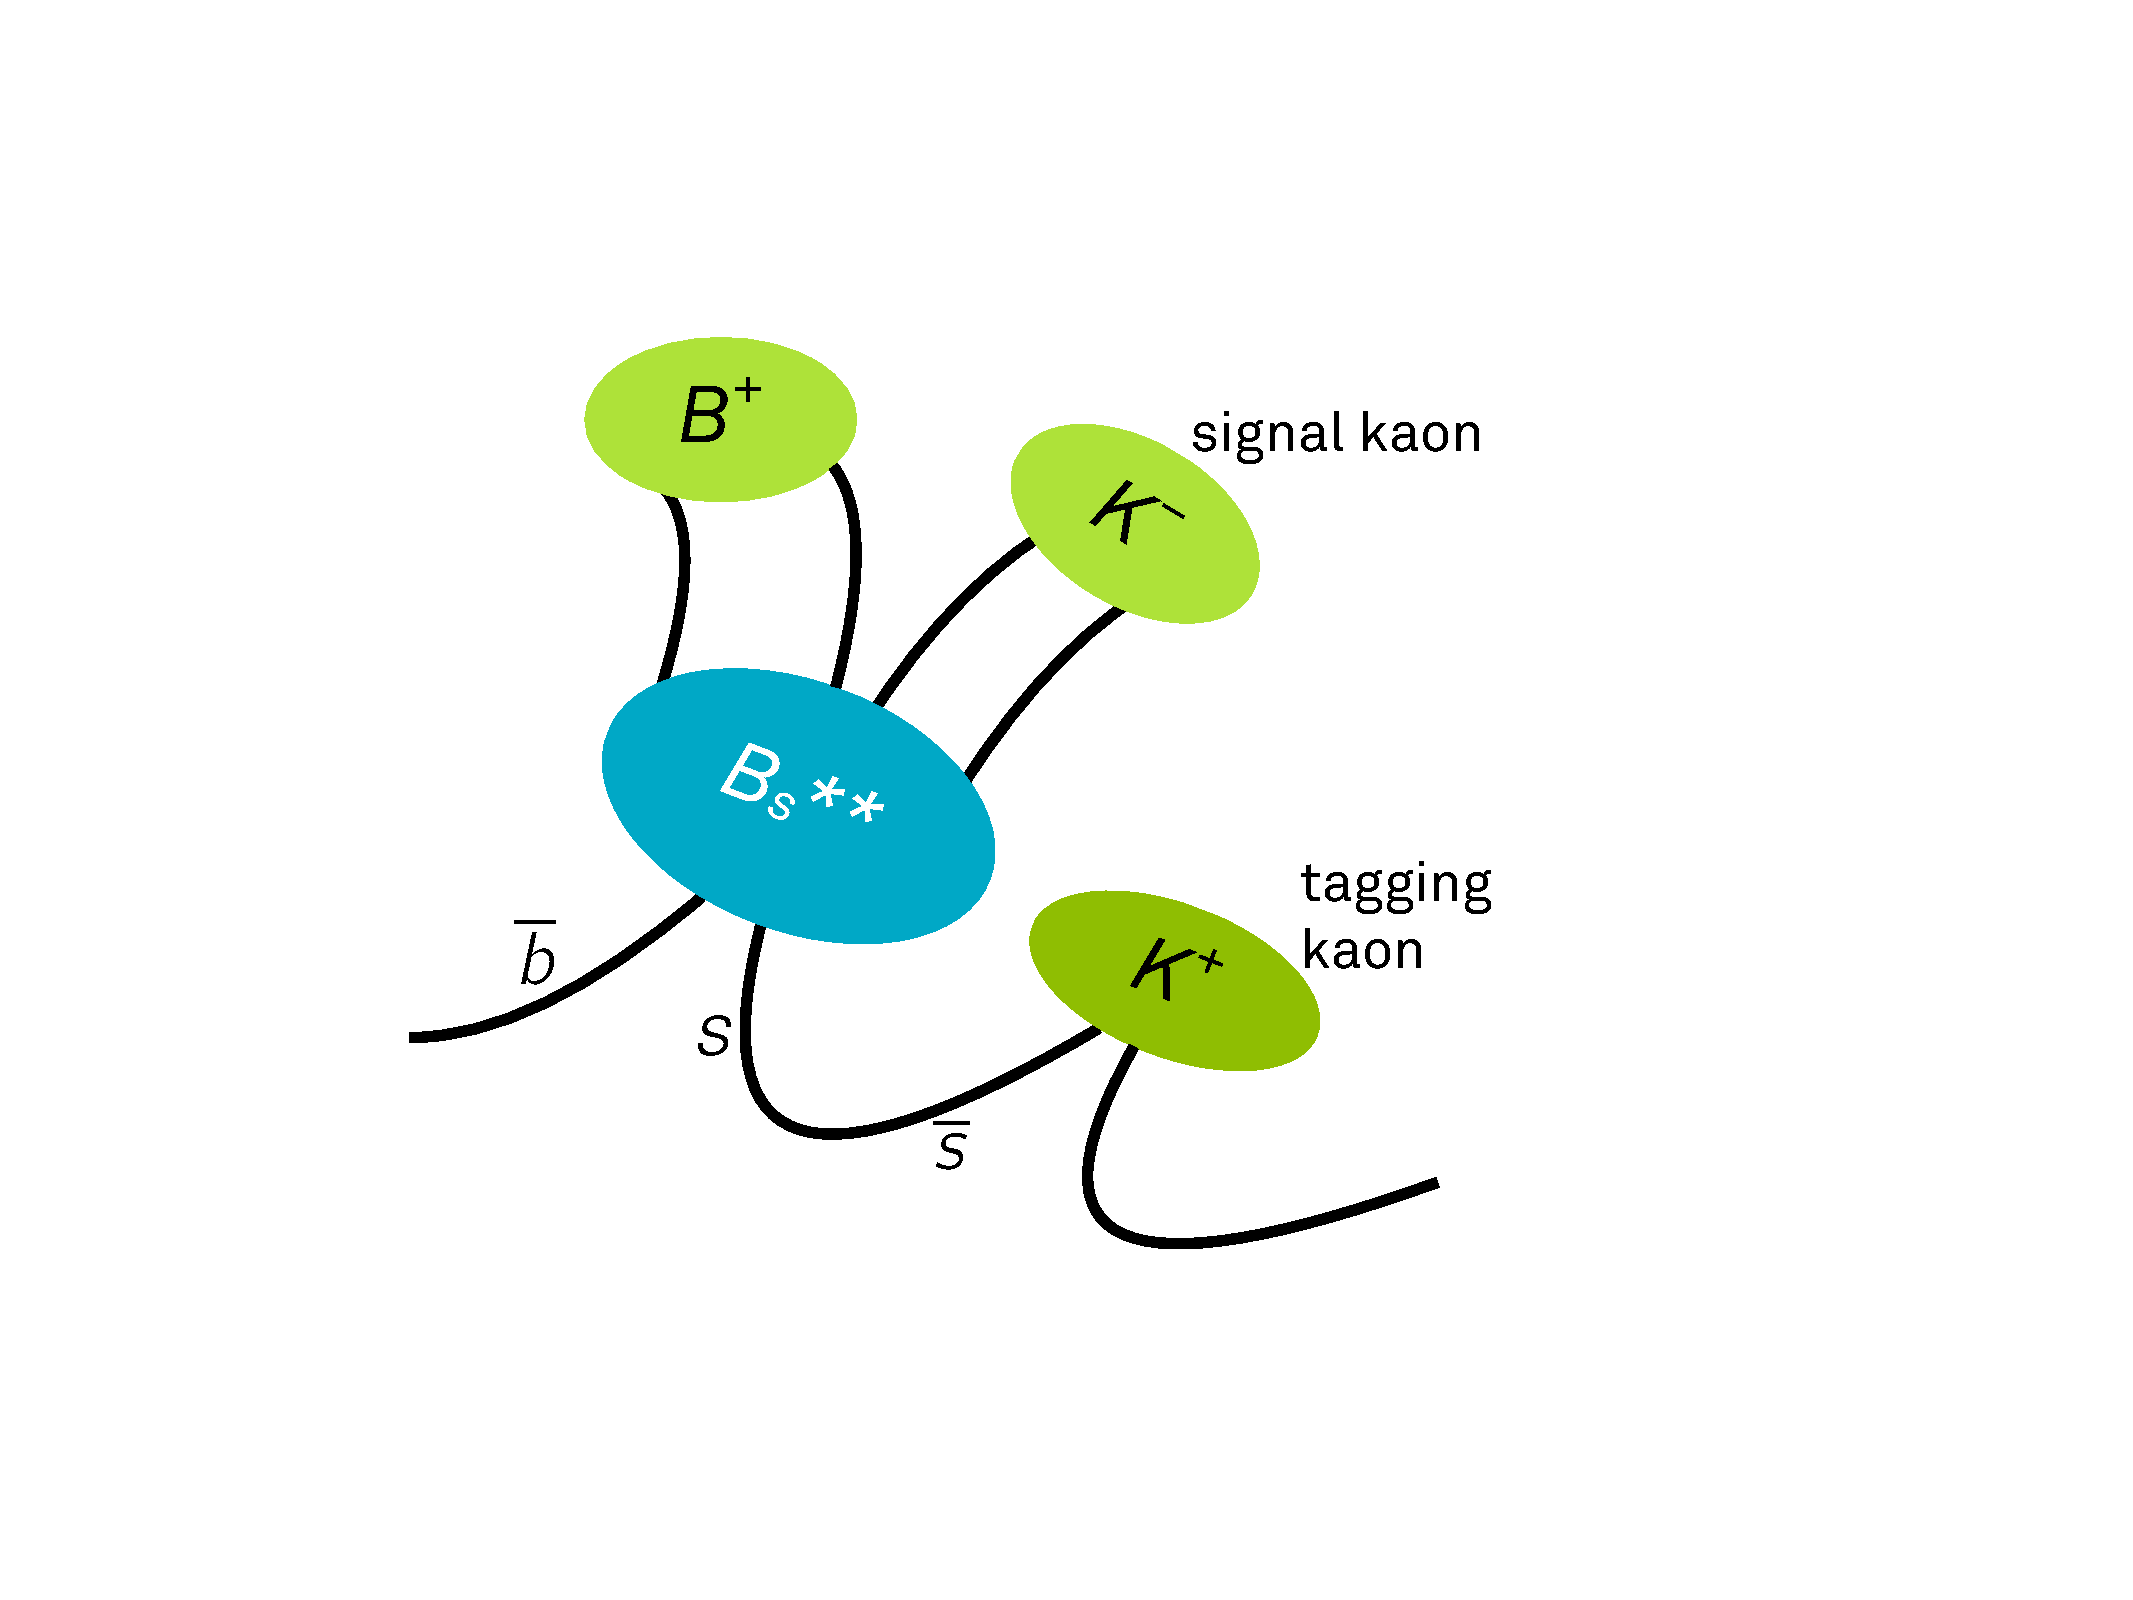
\includegraphics[width=0.608\textwidth]{figures/Bscalib.pdf}
\end{center}
\vspace{-1.7em}
\begin{itemize}
\setlength\itemsep{0.01em}
%\item further excited \Bs states are considered:
%\begin{itemize}
%\setlength\itemsep{0.01em}
%\setlength{\itemindent}{-.11in}
%\item[${\color{tu_gruen}-}$] $B_{s1}/B_{s2}^*\to B^{*+}K$
%\item[${\color{tu_gruen}-}$] add just few statistics
%\item[${\color{tu_gruen}-}$] missing \g from $B_{s1,2}^*\to\B\g$ is challenging
%\item[${\color{white}-}$] changes kinematic distributions of $B_{s1,2}$
%\end{itemize}
%\end{itemize}
%\begin{center}
%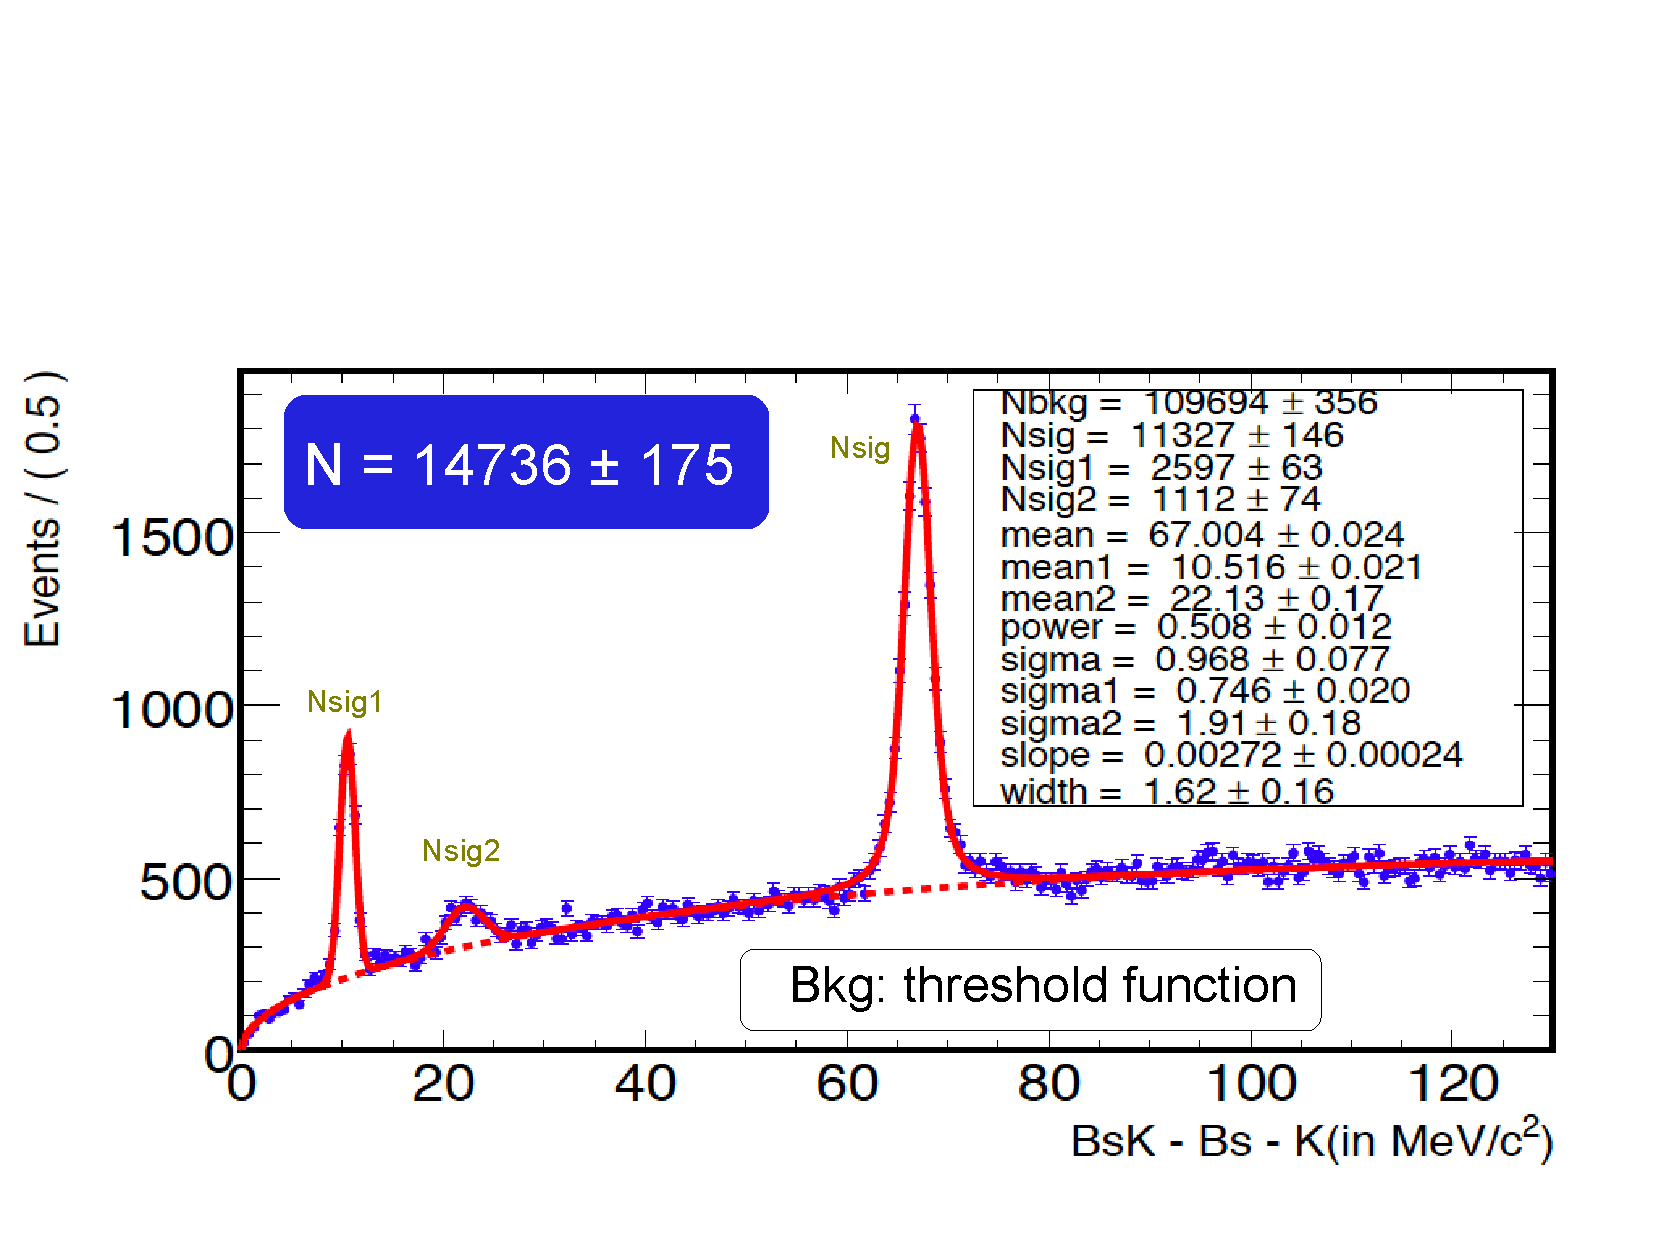
\includegraphics[width=\textwidth]{figures/BsdoublestarMass.pdf}%dürfen wir diesen Plot so zeigen?? -> ist aus dem PPTS Vortrag
%\end{center}
%\begin{itemize}
\item true independent crosscheck for \BsToDspi
\item results in agreement with \BsToDspi channel
%\item statistical uncertainties still limited
%\begin{equation*}
%\Delta p_0=0.002\pm0.011\hspace{0.5cm} \Delta p_1=-0.22\pm0.017 %ich weiß nicht ob wir diese Zahlen zeigen dürfen, vermute eher nicht
%\end{equation*}
%\vspace{-1.7em}
%\item analysis note in preparation
\end{itemize}

\vspace{0.1em}

\textbf{SS pion calibration}
\vspace{-0.1em}
\begin{itemize}
\setlength\itemsep{0.01em}
\item calibration performed with \BdToJPsiKst
\item full evaluation of systematic uncertainties 
%\begin{equation*}
%\begin{aligned}
%  p_0^{\text{SS\pion}}        &= \phantom{-}0.4232  \,\pm\, 0.0029           \text{\,(stat)} \,\pm\, 0.0020           \text{\,(syst)} \\ 
%  p_1^{\text{SS\pion}}        &= \phantom{-}1.011\phantom{0}   \,\pm\, 0.064\phantom{0} \text{\,(stat)} \,\pm\, 0.009\phantom{0} \text{\,(syst)} \\ 
%  \Delta p_0^{\text{SS\pion}} &= -0.0026 \,\pm\, 0.0043           \text{\,(stat)} \,\pm\, 0.0024           \text{\,(syst)}  \\
%  \Delta p_1^{\text{SS\pion}} &= -0.171\phantom{0}   \,\pm\, 0.096\phantom{0} \text{\,(stat)} \,\pm\, 0.029\phantom{0} \text{\,(syst)} \\
%  \langle\eta^{\text{SS\pion}}\rangle        &= \phantom{-}0.425\phantom{0} 
%\end{aligned}
%\end{equation*}
\item used for the first time in the measurements of
\begin{itemize}
\setlength{\itemindent}{-.11in}
\item[${\color{tu_gruen}-}$] $\sin(2\beta)$ with $\Bd \rightarrow \jpsi K_S^0$
\setlength{\itemindent}{.05in}
\item[${\color{tu_gruen}\Rightarrow}$] precision comparable to $B$-factories
\item[${\color{tu_gruen}\Rightarrow}$] $\varepsilon_{\text{eff}}^{\text{SS}\pion} = 0.38\,\%$
\setlength{\itemindent}{-.11in}
\item[${\color{tu_gruen}-}$] $\sin(2\beta_{\text{eff}})$ with $\Bd \rightarrow \jpsi \pi^+ \pi^-$
\setlength{\itemindent}{.05in}
\item[${\color{tu_gruen}\Rightarrow}$] $\varepsilon_{\text{eff}}^{\text{SS}\pion} = 0.54\,\%$
\end{itemize}


%\begin{equation*}
%\begin{aligned}
%&\Bd \rightarrow \jpsi K_S^0: &\varepsilon_{\text{eff}}^{\text{SS}\pion} &= 0.54\,\% \\
%&\Bd \rightarrow \jpsi \pi^+ \pi^-: &\varepsilon_{\text{eff}}^{\text{SS}\pion} &= 0.376\,\% 
%\end{aligned}
%\end{equation*}

\end{itemize}
\end{minipage}
\vspace{0.1em}
\hfill
\begin{minipage}{0.474\boxwidth}
\textbf{OS and SS Kaon tagging using neural nets (NN)}
\vspace{-0.1em}
\begin{itemize}
\item basic idea: use two NN
\begin{itemize}
\setlength\itemsep{0.01em}
\setlength{\itemindent}{-.11in}
\item[${\color{tu_gruen}-}$] first NN distinguishes between:
\begin{enumerate}
\item fragmentation tracks\\
${\color{tu_gruen}\Rightarrow}$ signal for SS kaon nnet
\item OS $b$ hadron tracks\\
${\color{tu_gruen}\Rightarrow}$ signal for OS kaon nnet
\item underlying event tracks 
\end{enumerate}
\end{itemize}
\vspace{-1.7em}
\begin{center}
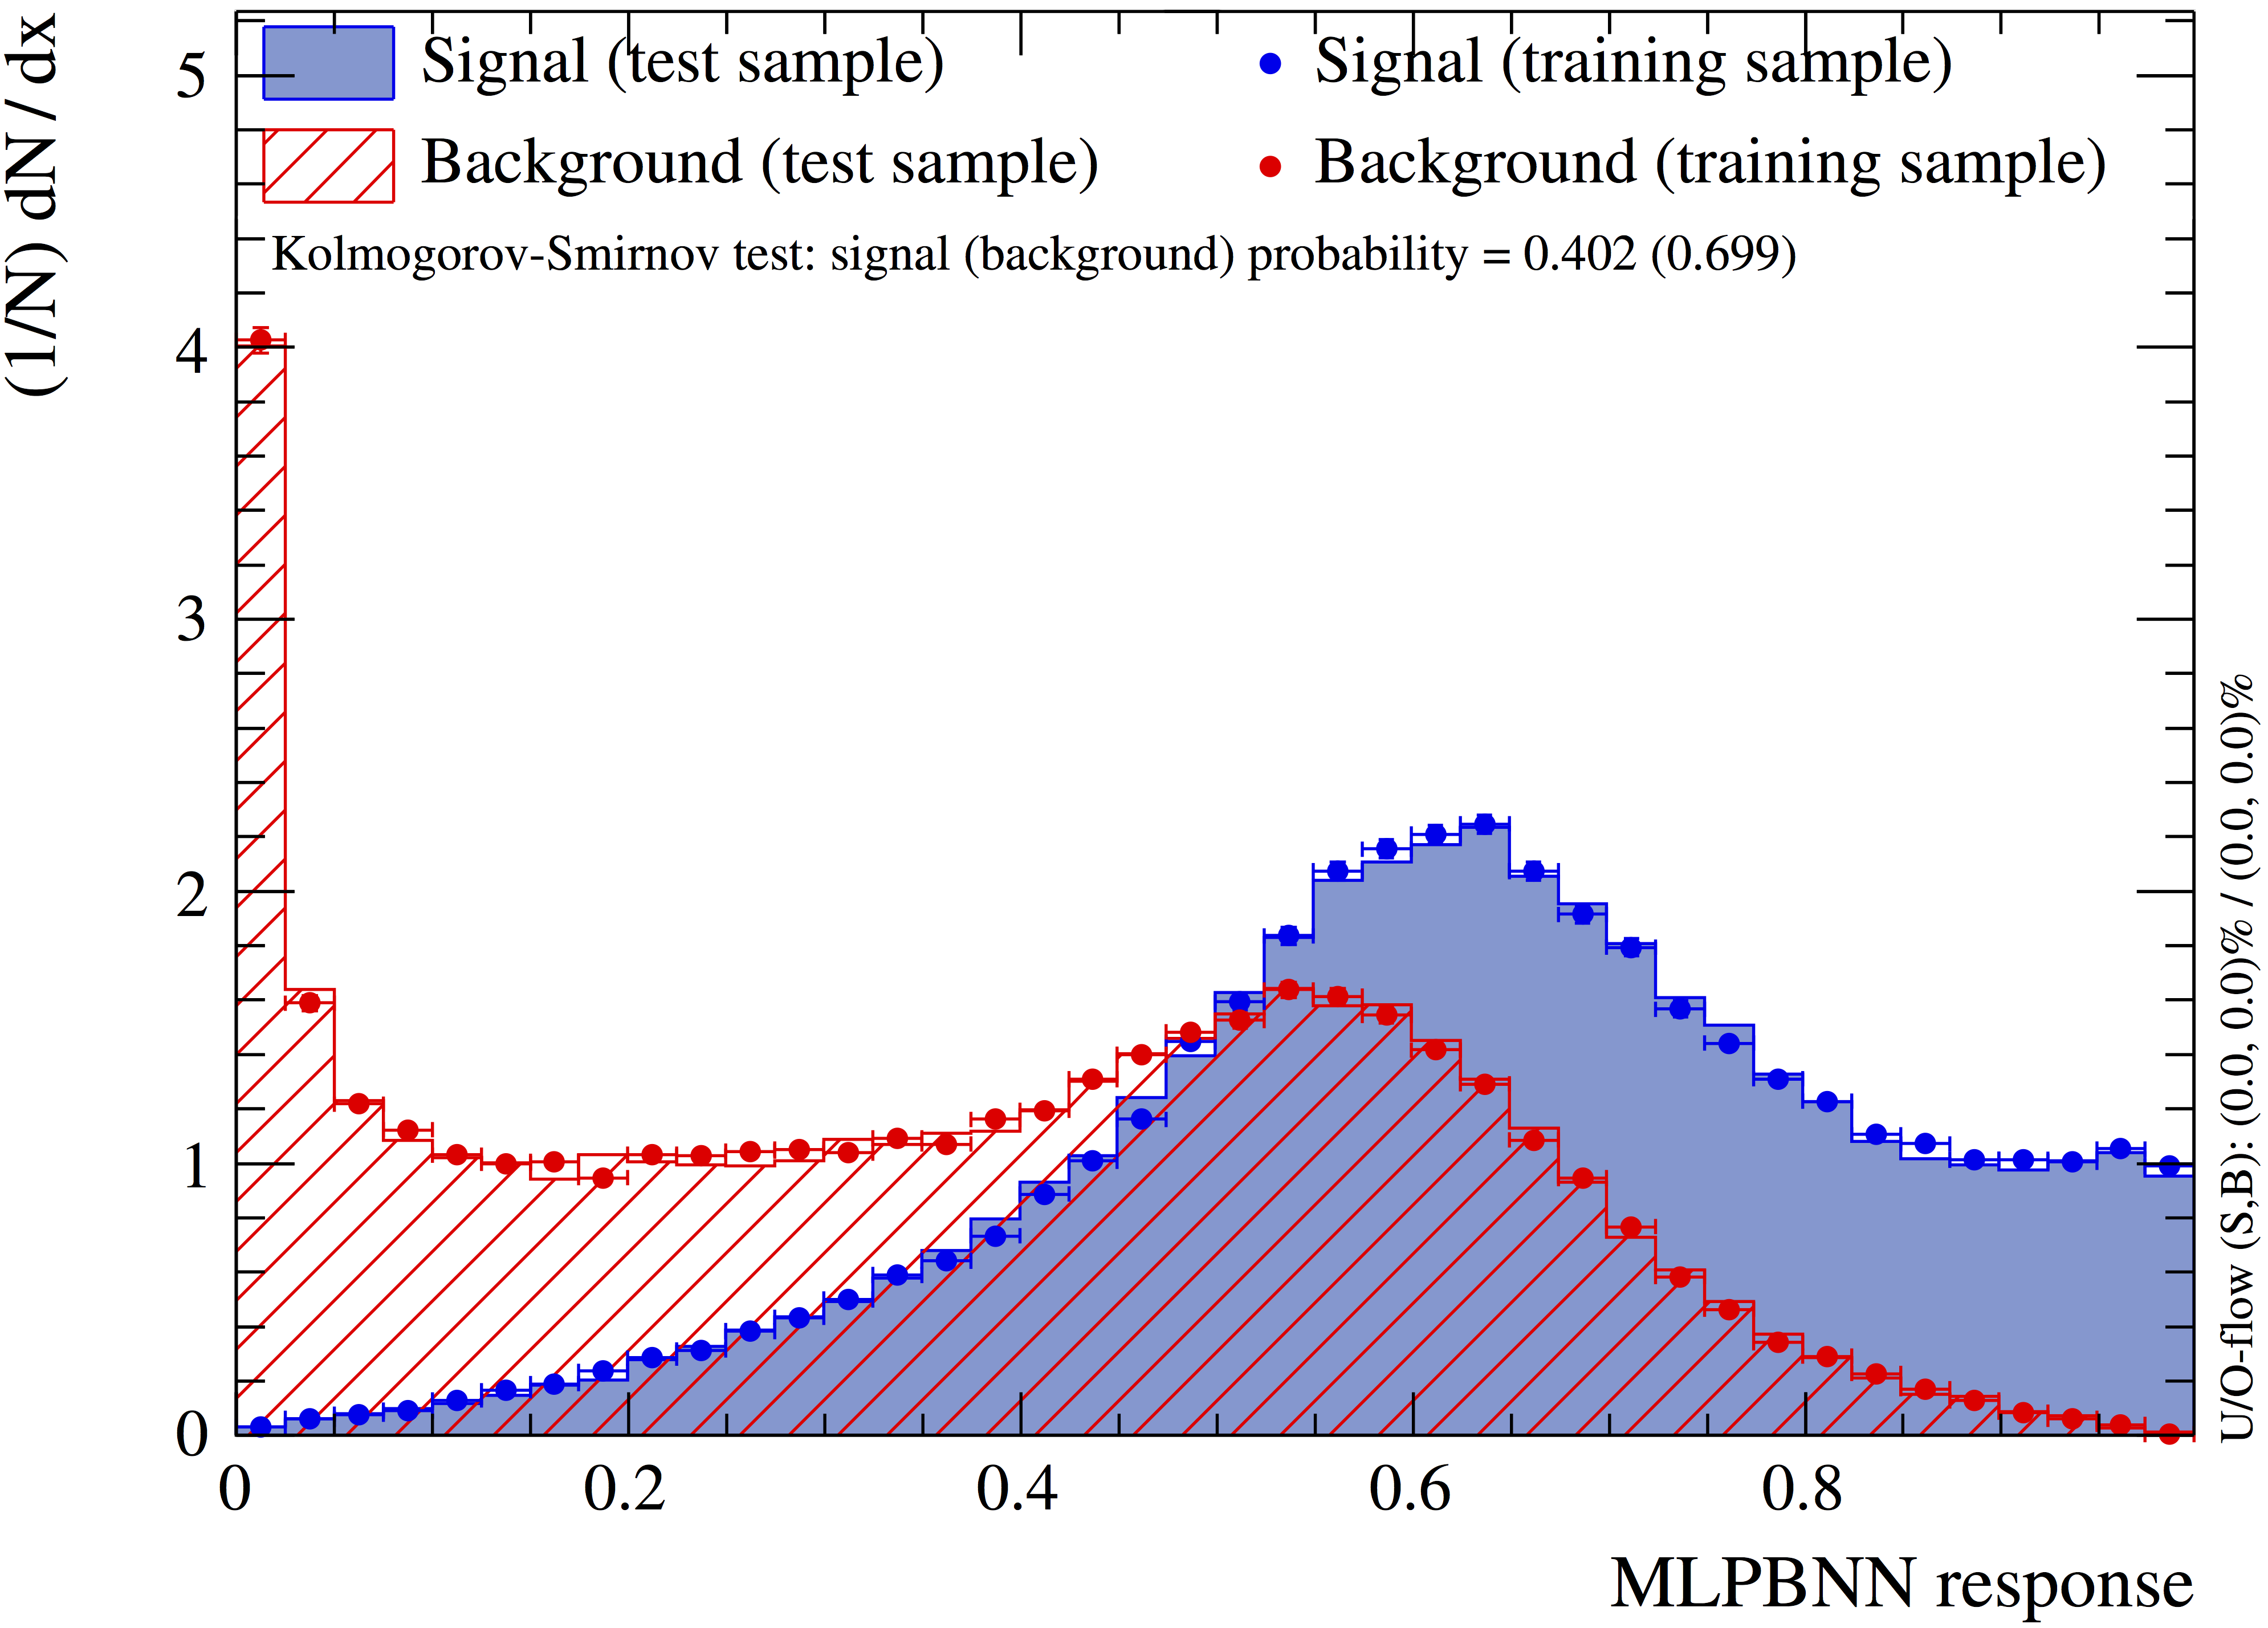
\includegraphics[width=0.802\textwidth]{figures/sskaonNnetfirstNN3.png}
\end{center}
\vspace{-2.5em}
\setlength\itemsep{0.01em}
\setlength{\itemindent}{-.11in}
\begin{itemize}
\setlength{\itemindent}{-.11in}
\item[${\color{tu_gruen}-}$] second NN:
\begin{itemize}
\item[${\color{tu_gruen}\circ}$] receives up to 3 candidates 
\item[${\color{tu_gruen}\circ}$] assigns final tag and mistag
\end{itemize}
\end{itemize}
\end{itemize}
\begin{itemize}
\setlength\itemsep{0.01em}
%\item both taggers have a high efficiency
\item SS kaon nnet tagger is a great success, compared \newline to the previous cut-based SS kaon it gives  
\begin{itemize}
\setlength{\itemindent}{-.11in}
\vspace{-0.5em}
\item[${\color{tu_gruen}-}$] \BsToDspi: $50\,\%$ relative improvement in $\varepsilon_{\text{eff}}$
\item[${\color{tu_gruen}-}$] \BsToJPsiPhi: $41\,\%$ relative improvement in $\varepsilon_{\text{eff}}$
\end{itemize}
%\item combined paper for both taggers in preparation
%\item SS kaon nnet:
%\begin{itemize}
%\setlength\itemsep{0.01em}
%\setlength{\itemindent}{-.11in}
%\item[${\color{tu_gruen}-}$] high mistag tagger: mean mistag O(43\%)
%\item[${\color{tu_gruen}-}$] compensating this with high statistics
%\item[${\color{tu_gruen}-}$] Improves tagging power by 40 \%
%\setlength\itemsep{0.01em}
%\setlength{\itemindent}{-.11in}
%\item[${\color{tu_gruen}-}$] improve selection of fragmentation tracks with neural network (trained on $\Bs\to\Ds\pi$)
%\item[${\color{tu_gruen}-}$] a second neural network, which computes the mistag and the tagging decision combines up to 3 multiple candidates
%\end{itemize}
%\begin{center}
%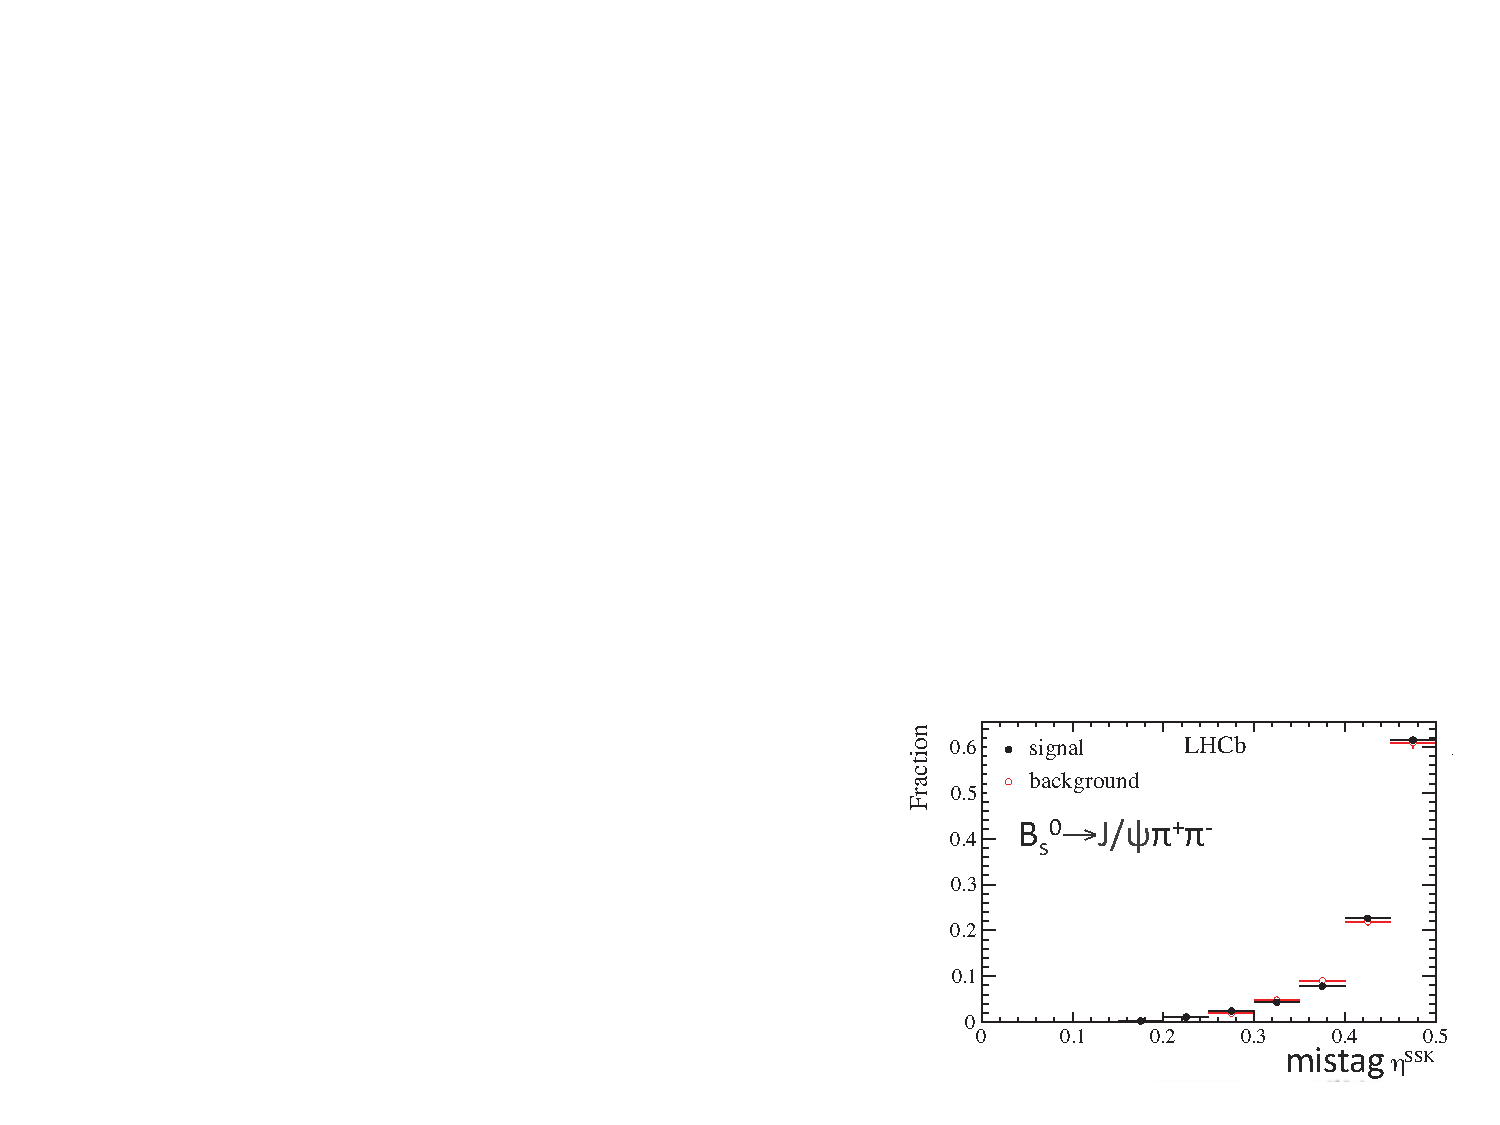
\includegraphics[width=0.8\textwidth]{figures/mistag_sskaonNN.pdf}
%\end{center}
\end{itemize}
\vspace{0.2em}
\textbf{OS charm tagger}
\vspace{-0.1em}
\begin{itemize}
\setlength\itemsep{0.01em}
\item reconstruct $D^0$/$D^\pm$/$D^*$ decays related to OS $b$ decay
\item one boosted decision tree (BDT) for each mode
\item clean measure of \B meson flavour (low mistag) 
\item adds about $0.37\,\%$ to $\epsilon_{\text{eff}}$
%\item analysis note in preparation
\end{itemize}
\vspace{0.3em}
\textbf{SS pion BDT and SS proton}
\vspace{-0.1em}
\begin{itemize}
\setlength\itemsep{0.01em}
\item promising new taggers based on BDT's
\item development ongoing
\end{itemize}
\vspace{-0.75em}
\end{minipage}
}




%combine NNet Tagger chapters